%!TEX TS-program = xelatex
\documentclass[12pt, a4paper, oneside]{article}

\usepackage{amsmath,amsfonts,amssymb,amsthm,mathtools}  % пакеты для математики

\usepackage[english, russian]{babel} % выбор языка для документа
\usepackage[utf8]{inputenc} % задание utf8 кодировки исходного tex файла
\usepackage[X2,T2A]{fontenc}        % кодировка

\usepackage{fontspec}         % пакет для подгрузки шрифтов
\setmainfont{Linux Libertine O}   % задаёт основной шрифт документа

\usepackage{unicode-math}     % пакет для установки математического шрифта
\setmathfont[math-style=upright]{Neo Euler} % шрифт для математики

% Конкретный символ из конкретного шрифта
% \setmathfont[range=\int]{Neo Euler}

\usepackage[paper=a4paper, top=5mm, bottom=5mm,left=5mm,right=5mm]{geometry}

%%%%%%%%%% Работа с картинками %%%%%%%%%
\usepackage{graphicx}                  % Для вставки рисунков
\usepackage{graphics}
\graphicspath{{images/}{pictures/}}    % можно указать папки с картинками
\usepackage{wrapfig}                   % Обтекание рисунков и таблиц текстом

%%%%%%%%%%%%%%%%%%%%%%%% Графики и рисование %%%%%%%%%%%%%%%%%%%%%%%%%%%%%%%%%
\usepackage{tikz, pgfplots}  % язык для рисования графики из latex'a

%%%%%%%%%% Гиперссылки %%%%%%%%%%
\usepackage{xcolor}              % разные цвета

\begin{document}

\begin{tikzpicture}
\node[inner sep=0pt] (russell) at (0,0)
{
\includegraphics[width=4.4cm,height=5.08cm]{rstudio.png}};
\node[inner sep=0pt] (russell) at (4.7,0)
{
\includegraphics[width=4.4cm,height=5.08cm]{rstudio.png}};
\node[inner sep=0pt] (russell) at (9.4,0)
{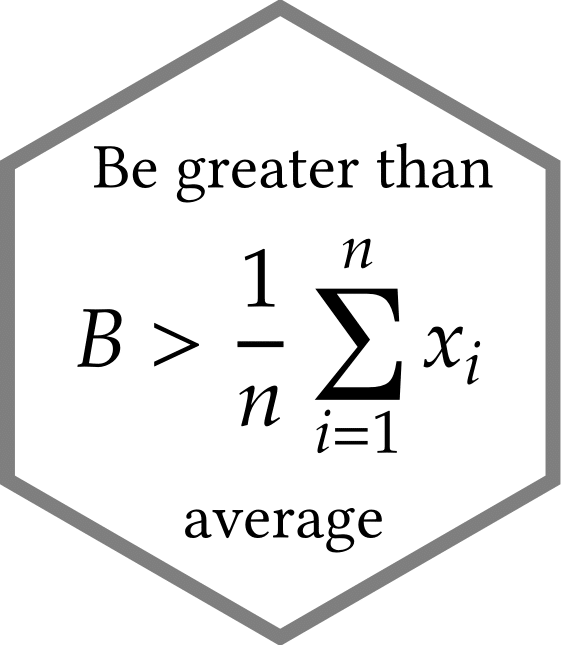
\includegraphics[width=4.4cm,height=5.08cm]{b+greater.png}};
\node[inner sep=0pt] (russell) at (14.1,0)
{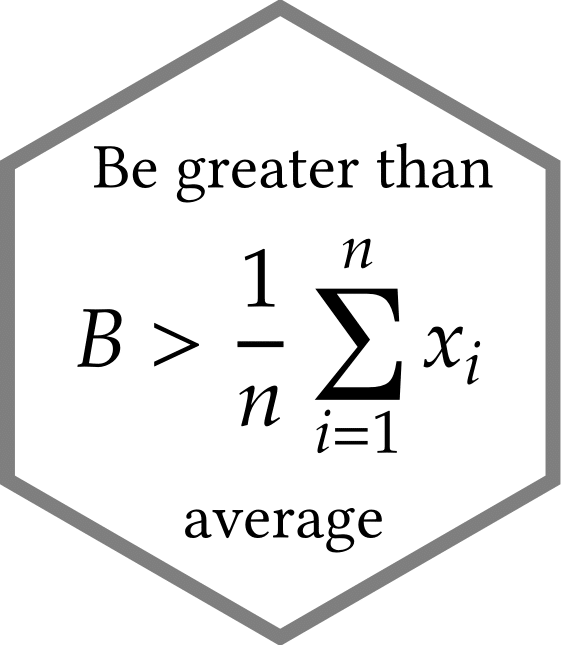
\includegraphics[width=4.4cm,height=5.08cm]{b+greater.png}};

\node[inner sep=0pt] (russell) at (0,-5.5)
{
\includegraphics[width=4.4cm,height=5.08cm]{potom_spat.png}};
\node[inner sep=0pt] (russell) at (4.7,-5.5)
{
\includegraphics[width=4.4cm,height=5.08cm]{potom_spat.png}};
\node[inner sep=0pt] (russell) at (9.4,-5.4)
{
\includegraphics[scale=0.165]{makro_mokro.png}};
\node[inner sep=0pt] (russell) at (14.1,-5.4)
{
\includegraphics[scale=0.165]{makro_mokro.png}};

\node[inner sep=0pt] (russell) at (0.3,-11)
{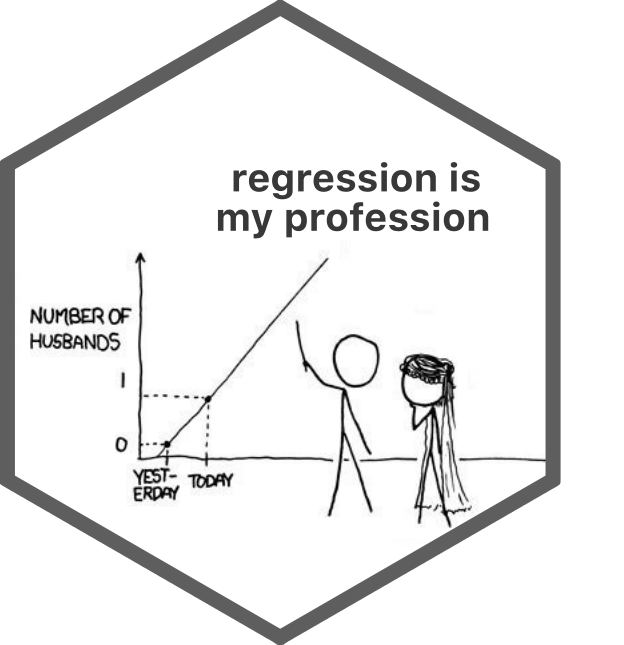
\includegraphics[scale=0.225]{regression_is_my.png}};
\node[inner sep=0pt] (russell) at (5,-11)
{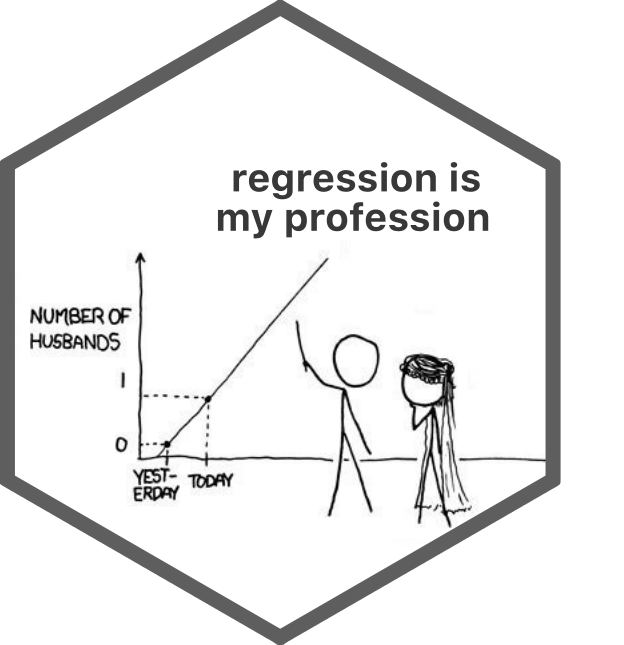
\includegraphics[scale=0.225]{regression_is_my.png}};
\node[inner sep=0pt] (russell) at (9.4,-11)
{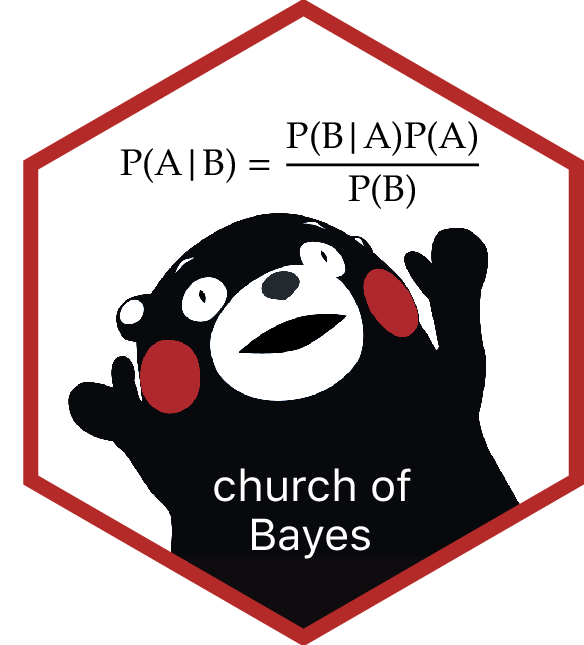
\includegraphics[width=4.4cm,height=5.08cm]{Bayes.png}};
\node[inner sep=0pt] (russell) at (14.1,-11)
{
\includegraphics[width=4.4cm,height=5.08cm]{zen.png}};

\node[inner sep=0pt] (russell) at (0,-16.5)
{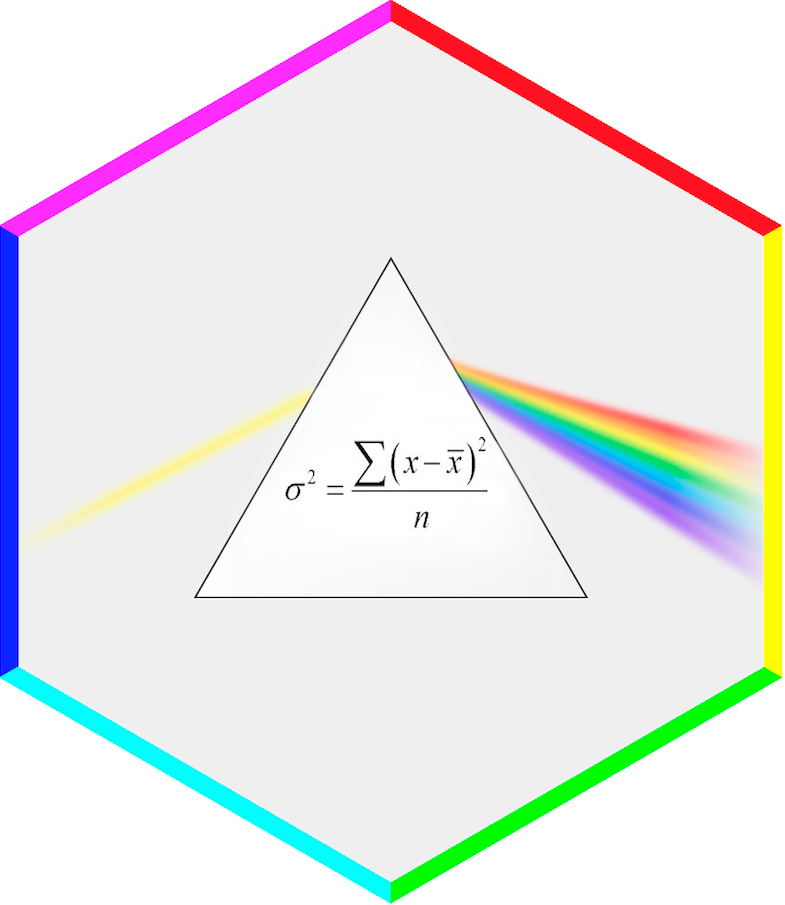
\includegraphics[width=4.4cm,height=5.08cm]{var.png}};
\node[inner sep=0pt] (russell) at (5,-16.5)
{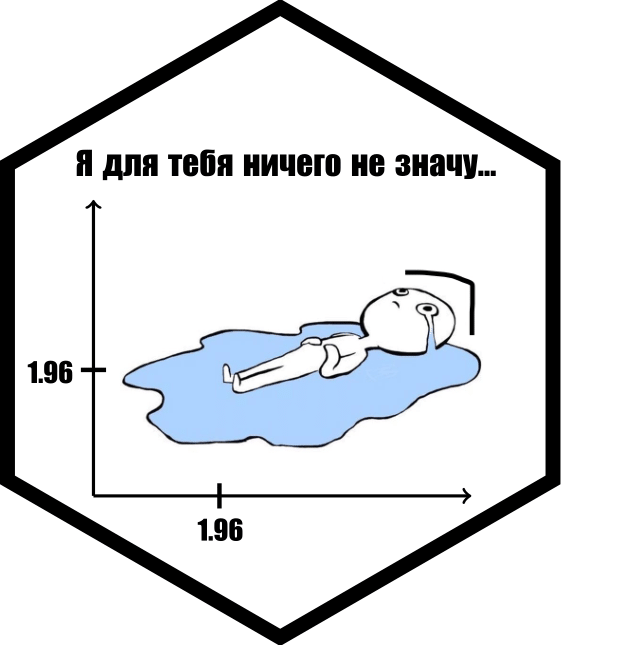
\includegraphics[scale=0.22]{elips.png}};
\node[inner sep=0pt] (russell) at (9.4,-16.5)
{
\includegraphics[width=4.4cm,height=5.08cm]{dummy_trap.png}};
\node[inner sep=0pt] (russell) at (14.1,-16.5)
{
\includegraphics[width=4.4cm,height=5.08cm]{beta_ek.png}};

\node[inner sep=0pt] (russell) at (0,-22)
{
\includegraphics[width=4.4cm,height=5.08cm]{mmmm_LaTeX.png}};
\node[inner sep=0pt] (russell) at (4.7,-22)
{
\includegraphics[width=4.4cm,height=5.08cm]{pot.png}};
\node[inner sep=0pt] (russell) at (9.17,-22.21)
{
\includegraphics[scale=1]{swan.png}};
\node[inner sep=0pt] (russell) at (14.1,-22)
{
\includegraphics[width=4.4cm,height=5.08cm]{wolfram.png}};


\end{tikzpicture}


% 
%
%
%
%
% 
%
%
%
% b+greater.png



\end{document} 